\section{Use-Cases}

\subsection{Use-case Diagram}
\begin{figure}
\centering
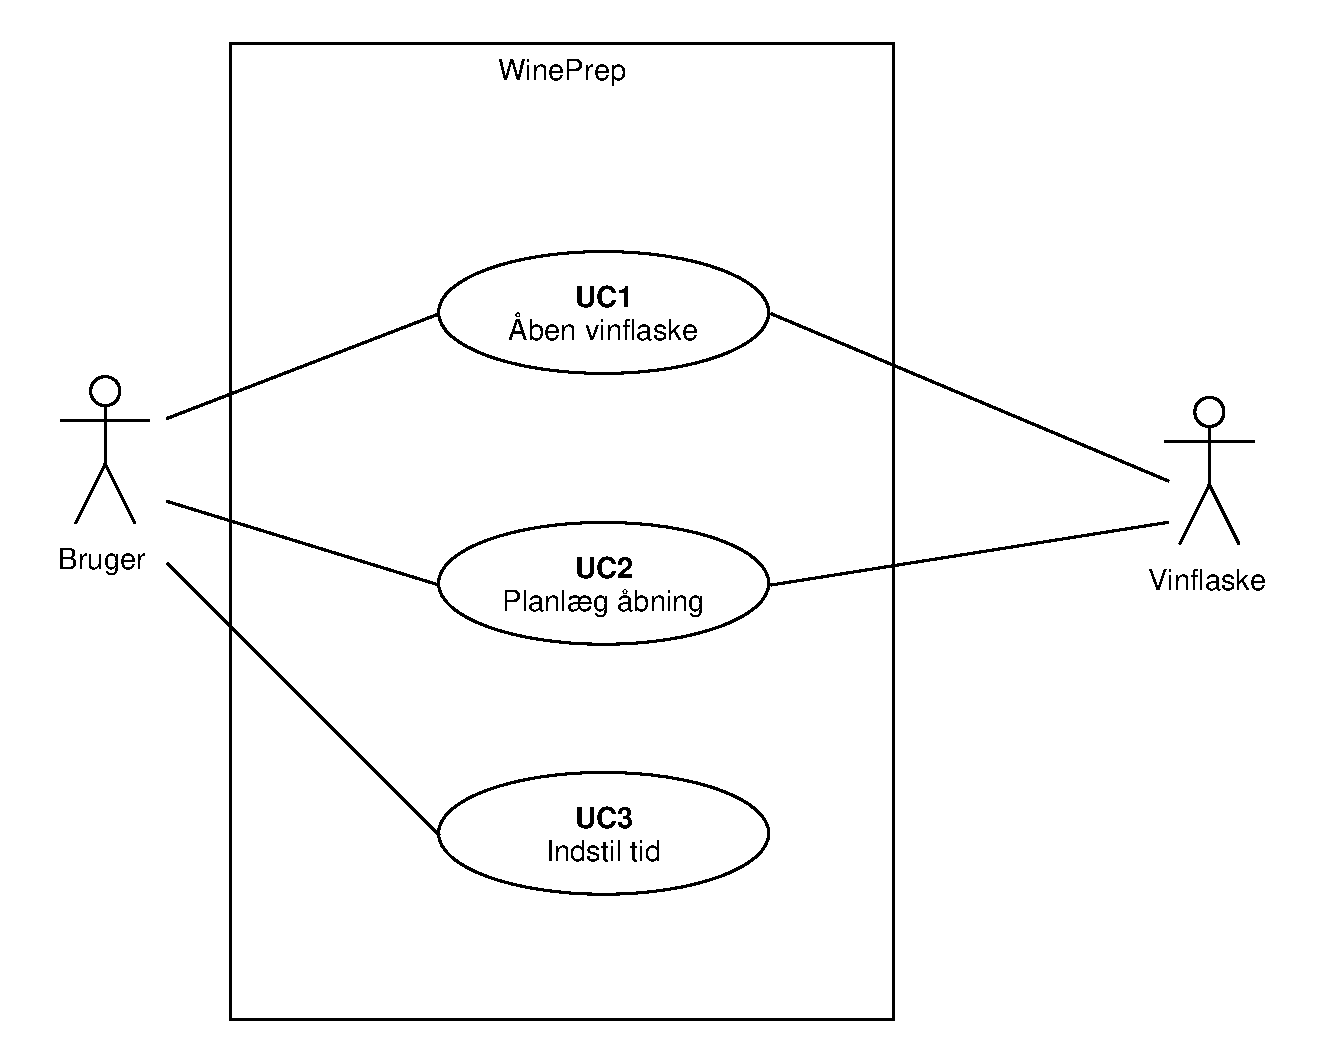
\includegraphics[scale=0.5]{usecasediagram.pdf}
\caption[Figur]{Usecase Diagram}
\end{figure}
\newpage
\subsection{Use-case 1: Åbn Vin}
\rowcolors{1}{white}{lightgray}
\begin{tabular}{>{\bfseries}p{100pt} p{300pt}}
%	\caption[Tabel]{Fully dressed use-case 1}
	Navn & \bfseries{UC 1: Åbn Vinflaske} \\
	Mål & At åbne vinflasken og dermed tillade brugeren adgang til vinen\\
	Initiering & test 2 \\
	Aktører & Primær: Bruger \\
	Antal Samtidige forekomster & 1 \\
	Prækondition & Vinflasken er anbragt i systemet og systemet er klar til brug. Desuden er vinflasken uåbnet og forseglingen er fjernet. \\
	Postkondition & Vinflasken er åbnet \\
	Hovedscenarie & \begin{enumerate}
		\item System detektere vinflaskens type og position
		\subitem [Ext. 1: System registrerer ugyldig type af vinflaske]
		\subitem [Ext. 2: System kan ikke registrere en vinflaske] 
		\item System låser vinflasken i dens position
		\item System fjerne prop fra vinflasken
		\item System frigiver vinflasken
		\item System meddeler brugeren om at vinflasken er åbent og klar til brug.
		\item System dispenserer prop.
	\end{enumerate} \\
	Udvidelser/Undtagelser & 
	\begin{enumerate}{}{}
	\item[Ext.1] System registrerer ugyldig type af vinflaske
	
		\subitem[1.1] System meddeler brugeren om at typen af vinflaske er ugyldig.
		\subitem[1.2] UC1 Afsluttes.
	\item[Ext.2] System kan ikke registrere en vinflaske
		\subitem[2.1] {System meddeler brugeren om at ingen vinflaske \newline er
		registreret
}
		\subitem[2.2] UC afsluttes
	\end{enumerate}\\
\end{tabular}



\subsection{Use-case 2: Planlæg Åbning}
\rowcolors{1}{white}{lightgray}
\begin{tabular}{>{\bfseries}p{100pt} p{300pt}}
	
	Navn & \bfseries{UC 2: Planlæg Åbning} \\
	Mål & Vinen er drikkeklar til et forudbestemt tidspunkt\\
	Initiering & Bruger trykker \emph{Planlæg Åbning} på brugergrænsefladen\\
	Aktører & Primær: Bruger \\
	Antal Samtidige forekomster & 1 \\
	Prækondition & Vinflasken er anbragt i systemet og systemet er klar til brug. Desuden er vinflasken uåbnet og forseglingen er fjernet. \\
	Postkondition & Vinflasken er drikkeklar til det valgte tidspunkt\\
	Hovedscenarie & \begin{enumerate}
		\item Bruger vælger tidspunkt på systemet
		\subitem [Ext. 1: Bruger ønsker ikke at åbne vin] 
		\item Bruger bekræfter valgt tidspunkt
		\subitem [Ext. 2: Vinen kan ikke iltes korrekt til det valgte tidspunkt]
		\item System venter til iltningstidspunktet
		\subitem [Ext. 3: System registrererugyldig type af vinflaske]
		\item System detekterer vinflaskens type og position
		\subitem [Ext. 4: System registrerer ugyldig type af vinflaske]
		\subitem [Ext. 5: System kan ikke registrere en vinflaske]
		\item System låser vinflasken i dens position
		\item System fjerner prop fra vinflasken
		\item System frigiver vinflasken
		\item System dispenserer prop
		\item System venter til, at vinen er drikkeklar
		\item System meddeler brugeren om, at vinen er drikkeklar		
	\end{enumerate} \\
	Udvidelser/Undtagelser & 
	\begin{enumerate}{}{}
		\item[Ext.1] \bfseries{ Bruger ønsker ikke at åbne vin} 
		
		\subitem[1.1a] Bruger trykker på \emph{Tilbage}
		\subitem[1.2b] UC afsluttes
		\item[Ext.2] \bfseries{ Vinen kan ikke iltes korrekt til det valgte tidspunkt}
		\subitem[2.1] System beder bruger bekræfte valg af tidspunkt
		\subitem[2.2a] Bruger trykker bekræft
		\subitem[2.3a] UC fortsættes fra punkt 1 i UC 1
		\subitem[2.2b] bruger trykker \emph{Annuller}
		\subitem[2.3b] UC afsluttes
		\item[Ext.3] \bfseries{ Bruger annullerer planlagt åbning af vin}
		\subitem[3.1] Bruger trykker \emph{STOP!}
		\subitem[3.2] System beder bruger bekræfte valg
		\subitem[3.3a] Bruger trykker \emph{Bekræft}
	\end{enumerate}
\end{tabular}